
\section{Diskrete Modelle}

\begin{Definition}[Laplace Wahrscheinlichkeit]
Sei $\Omega = \{ \omega_1, \cdots , \omega_n\}$ eine endliche Menge. Für $A \subset \Omega$ definieren wir die Wahrscheinlichkeit durch
\begin{align*}
P(A) : = \frac{\#A}{ \# \Omega} \; . 
\end{align*} 
Die Elemente $ \omega_1, \cdots , \omega_n \in \Omega$ nennen wir Elementarereignisse und Teilmengen $A \subset \Omega$ Ereignisse. Die Abbildung
\begin{align*}
P : \mathcal{P} (\Omega) \to [0,1]  
\end{align*}  
nennen wir die Laplace-Verteilung bzw. Gleichverteilung auf $\Omega$.
\end{Definition}


\begin{Definition}[Permutationen und Kombinationen]

\begin{itemize}
\item $Perm_k^n(\Omega, m.W.) : = \{ \omega_1, \ldots, \omega_k \in \Omega^k \}$  Menge aller Permutationen mit Wiederholung.
\item $Perm_k^n(\Omega, o.W.) : = \{ \omega_1, \ldots, \omega_k \in \Omega^k  | \omega_i \neq \omega_j\}$  Menge aller Permutationen ohne Wiederholung.
\item $Kom_k^n(\Omega, m.W.) : = \{ \omega_{i_1}, \ldots, \omega_{i_k} \in \Omega^k  | 1  \leq i_1 \leq  \ldots  \leq i_k \}$  Menge aller Kombinationen  mit Wiederholung.
\item $Kom_k^n(\Omega, o.W.) : = \{ \omega_{i_1}, \ldots, \omega_{i_k} \in \Omega^k  | 1 \leq i_1  \leq \ldots \leq i_k ;  \omega_{i_i} \neq \omega_{i_j} \}$  Menge aller Kombinationen  ohne  Wiederholung.
\end{itemize}
\end{Definition}

\begin{Lemma}
\begin{itemize}
\item $\# Perm_k^n(\Omega, m.W.)  = n^k = \underbrace{n \cdot n \cdots n}_{\text{k-mal}}$
\item $\# Perm_k^n(\Omega, o.W.)  = n_k = n \cdot (n-1) \cdots  (n-(k-1)) = \frac{n!}{(n-k)!}$  
\item $\#Kom_k^n(\Omega, o.W.) = \binom{n}{k} = \frac{n!}{k! (n-k)!}$  
\item $\#Kom_k^n(\Omega, m.W.)  = \binom{n + k -1}{k}$  
\end{itemize}
\end{Lemma}
\begin{proof}
\end{proof}


\begin{Definition}{Diskrete Wahrscheinlichkeitsverteilung}
Es sei $\Omega$ eine (nicht leere) albzählbare Menge. Eine Abbildung 
$P :\mathcal{P}(\Omega) \to [0,1]$ heißt diskrete Wahrscheinlichkeitsverteilung (Wahrscheinlichkeismaß), falls gilt:
\begin{align*}
& P(\Omega) = 1\\
& P \Biggl( \bigcup_{n=1}^{\infty} A_n \biggr)= \sum_{n=1}^{\infty} P(A_n), \text{ mit } A_i \cap A_j = \emptyset \text{ für } i \neq j 
\end{align*}
\end{Definition}


\begin{Beispiel}{Beispiel: Laplace Wahrscheinlichkeit}
$\Omega$ endlich und $P(A) = \frac{\#A}{\#\Omega}$.
 \end{Beispiel}


\begin{Definition}{Bedingte  Wahrscheinlichkeit}
Für $A,B \subset \mathcal{P}(\Omega)$ und $P(B) > 0$ heißt
\begin{align*}
& P(A \; | \;  B) = \frac{P(A \cap B)}{P(B)} \\
\end{align*}
die bedingte Wahrscheinlichkeit (von $A$ unter $B$).
\end{Definition}


\begin{figure}[htp]
      \centering
    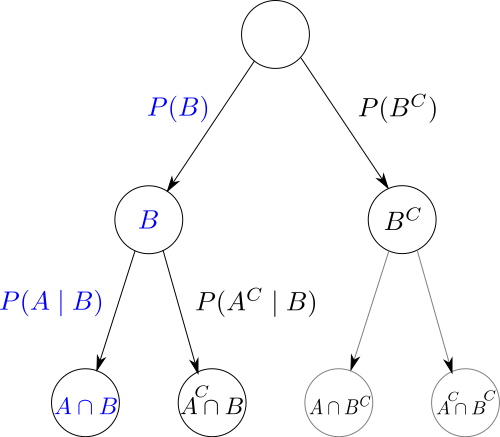
\includegraphics[width=0.5\textwidth]{images/Probability_tree}

      \caption{Quelle: Wikipedia}
\end{figure}



\begin{Satz}{Satz der totalen Wahrscheinlichkeit}
Für eine Zerlegung  $\Omega = \bigcup_{j=1}^{n} B_j, \text{ mit } B_i \cap B_k = \emptyset \text{ für } i \neq k $
\begin{align*}
& P(A ) = \sum_{j=1}^{n}  P(A \; | \;  B_j) \cdot P(B_j)
\end{align*}
\end{Satz}
\begin{proof}
$A = A \cap B \cup A \cap \bar{B}$ und  $A \cap B \cap A \cap \bar{B} = \emptyset$. 
\begin{align*}
& P(A) =  P(A \cap B) + P(A \cap \bar{B}) = P(B) \cdot P(A  \; | \; B) + P(\bar{B}) \cdot P(A  \; | \; \bar{B}) 
\end{align*}
\end{proof}

\begin{Satz}{Satz von Bayes}
Für $A,B \subset \mathcal{P}(\Omega)$ mit  $P(B) > 0$ gilt
\begin{align*}
& P(A \; | \;  B) = \frac{P(B \; | \; A) \cdot P(A)} {P(B)} \\
\end{align*}
\end{Satz}

\begin{proof}
\begin{align*}
& P(A \; | \;  B) =\frac{P(A \cap B)}{P(B)} = \frac{ \frac{P(A \cap B) \cdot P(A)}{P(A)}}{P(B)}  =  \frac{P(B \; | \; A) \cdot P(A)} {P(B)} 
\end{align*}
\end{proof}


\begin{Definition}{Stochastische Unabhängigkeit}
Zwei Ereignisse $A,B$ heißen stochastisch Unabhängig, falls
\begin{align*}
P(A \cap B) = P(A) \cdot P(B)
\end{align*}
gilt.  Somit ist auch $P(A | B) = P(A)$ und $P(B  | A) = P(B)$.
\end{Definition}


\subsection{Naiver Bayes'scher Spam Filter}
Gegeben ist eine E-Mail $E$.  Wir möchten anhand des Vorkommens bestimmter Wörter $A_1, \ldots A_n$ in der Mail entscheiden, ob es sich um eine erwünschte Mail $H$ oder eine unerwünschte Mail $S$ (Ham or Spam) handelt. 
(Typische Wörter wären zum Beispiel "reichwerden",  "onlinecasino" ...)
Aus einer Datenbank kann man das Vorkommen dieser Wörter in Spam und Ham Mails zählen und damit empirisch die Wahrscheinlichkeiten $P(A_i | S)$ und $P(A_i | H) $ des Vorkommens dieser Wörter in Spam und Ham Mails ermitteln.  Wir gehen davon aus, dass es sich bei der Mail  prinzipiell mit  Wahrscheinlichkeit $P(E= S) = P(E= H)= \frac{1}{2}$  um eine erwünschte  Mail $H$ oder eine unerwünschte Mail $S$  handeln kann. 




 Wir machen zudem die (naive) Annahme, dass das Vorkommen der Wörter  stochastisch unabhängig ist, also 
\begin{align*}
P(A_1 \cap \cdots \cap A_n | S) = P(A_1 | S) \cdots P(A_n | S) \\
P(A_1 \cap \cdots \cap A_n | H) = P(A_1 | H) \cdots P(A_n | H)
\end{align*}
gilt.


Mit der Formel von Bayes und der totalen Wahrscheinlichkeit  können wir somit berechnen
\begin{align*}
& P(E=S |  A_1 \cap \cdots \cap A_n) = \frac{P(A_1 \cap \cdots \cap A_n | S) \cdot P(S)}{P(A_1 \cap \cdots \cap A_n)} \\
&=  \frac{P(A_1 | S) \cdots P(A_n | S) \cdot P(S)}{P(A_1 \cap \cdots \cap A_n | H) + P(A_1 \cap \cdots \cap A_n | S)} \\
&=  \frac{P(A_1 | S) \cdots P(A_n | S) \cdot P(S)}{P(A_1 | H) \cdots P(A_n | H)  + P(A_1 | S) \cdots P(A_n | S) } \\
\end{align*}
Bemerkung: $P(E=H |  A_1 \cap \cdots \cap A_n) = 1- P(E=S |  A_1 \cap \cdots \cap A_n) $





